%\begin{flushright}
%%%\emph{``For the things we have to learn before we can do them, we learn by doing them.''}\\%Each wrong scenario you have analysed, is a wrong decision you won't made.''}\\
%%%Aristote
%\emph{All models are wrong, but some are useful.}\\
%George P. Box
%\end{flushright}

%\medskip
%
%\begin{mybox}{Chapter overview}
%\begin{itemize}[left=0em]%[leftmargin=0cm,itemindent=.5cm,labelwidth=\itemindent,labelsep=0cm,align=left]
%\setlength\itemsep{-0.3em}
%\item Belgian energy system overview%Case studies: the Belgian energy systems during the transition (2015-2050).
%\end{itemize}
%\vspace{-0.3cm}
%
%\emph{This chapter is an improved and extended case study version of \citet{Limpens_belgian_2020}}.
%\end{mybox}
%
%\medskip

\section{Contributions}
\label{sec:meth:contributions}
\begin{itemize}
\item Apply Stefano's method on the pathway model with a similar approach as Guevara et al.
\item Check that PCE was appropriate as a method for such a system (ECOS2020)
\item Work on the $C_inv_return$
\end{itemize}

\section*{Other authors' main contribution statement}
On top of the main contributions of this thesis that are aforementioned, three main authors are to be mentioned for having brought a significant part of the methodological work. Based on Stefano Moret's monthly whole-energy system model (\ie EnergyScope) \cite{moret2016strategic}, Gauthier Limpens has developed the hourly version of the snapshot model (\ie EnergyScope TD) \cite{limpens2019energyscope}, as well as the perfect foresight pathway model \cite{limpens2024pathway}, to which I personally contributed too. Diederik Coppitters has developed the RHEIA framework allowing to quantify the impact of uncertainties and carry out robust optimisation of energy systems \cite{coppittersthesis}. The current work used this framework for the first of these functionalities. Finally, Stefano Moret extensively assessed the uncertainty characterisation on the Swiss energy system \cite{Moret2017}. This thesis follows the same methodology, updating the uncertainty ranges for the pathway model.

\section{Whole-energy system transition model optimisation: EnergyScope Pathway}
\label{sec:meth:ES}

On the contrary, this work optimises the entire transition pathway from a known system in 2020 up to 2050 thanks to EnergyScope Pathway \cite{limpens2024pathway}. According to pathway models review (see Appendix \ref{app:ESPathway_choice}), EnergyScope Pathway can be categorised as an investment and operation optimisation model that assesses the whole-energy system, has a hourly time-resolution and is open-source documented model. Moreover, it maintains a low computational cost (\ie around 15 minutes for a 30-year pathway with a hourly discretisation). From the perfect to the myopic foresight of the transition optimisation, this section presents only the main constraints of the model. The reader is invited to refer to Appendix \ref{app:ESPathway_full_formulation} for more details about the formulation of the model and its extension from a snapshot approach, EnergyScope TD. More extensive information about the formulation choices, for instance, can be found in \cite{limpens2024pathway} and the documentation \cite{readthedocs_pathway}.

\begin{figure}[htbp!]
\centering
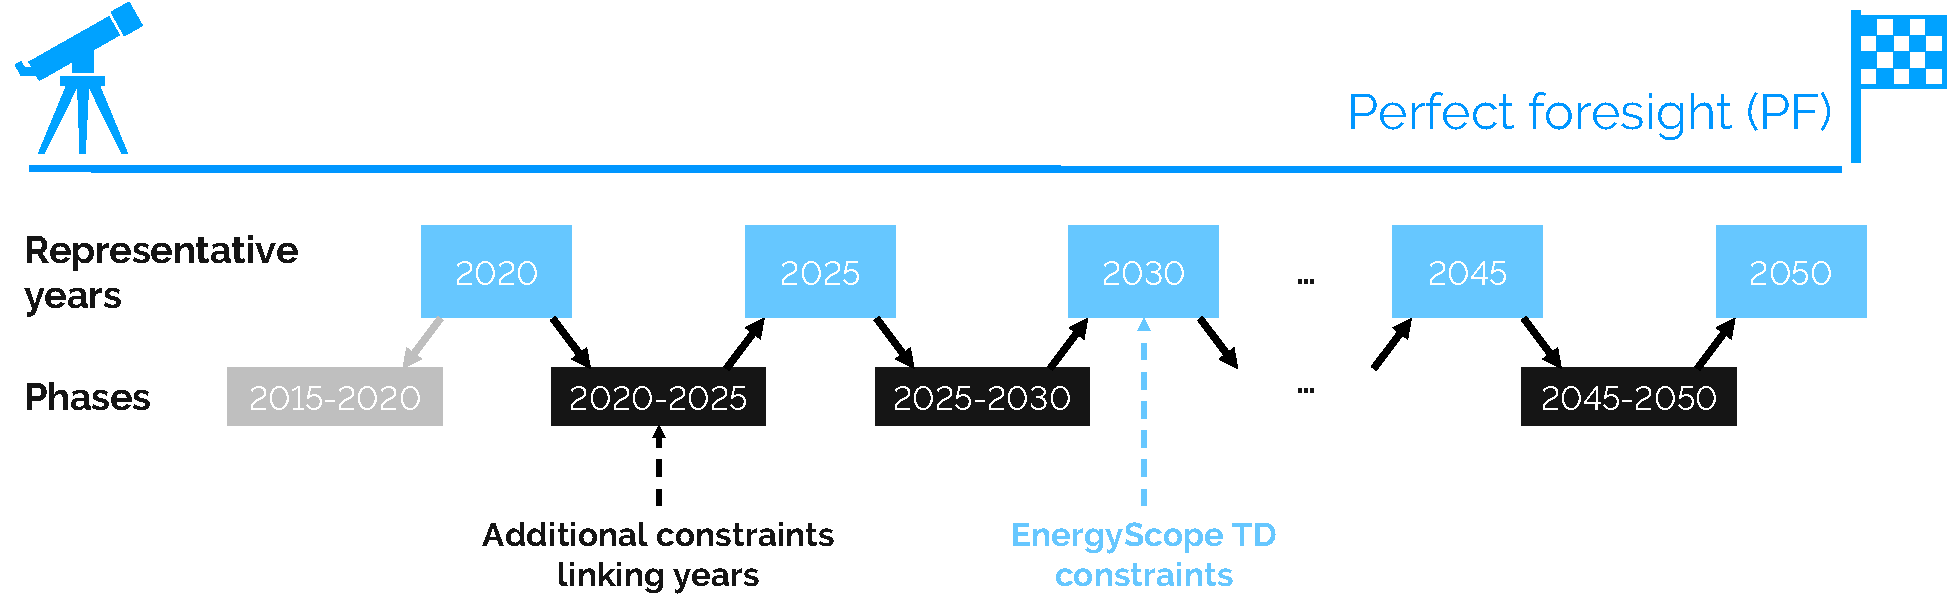
\includegraphics[width=\textwidth]{ES_Pathway.pdf}
\caption{Illustration of the pathway methodology based on an existing energy system model. The methodology spans from 2020 to 2050, with one representative year every five years. The model \acrfull{ESTD} is applied in 7 representative years (light blue boxes). The formulation includes additional constraints (black boxes) that link the years together. The pathway's initialisation assumes that all capacities installed in 2020 were built during the pseudo-phase of 2015-2020 (grey box). The overall problem is defined as the pathway model.}
\label{fig:meth_path_methodology_core}
\end{figure}

We used the perfect foresight (PF) formulation (\Cref{fig:meth_path_methodology_core})---the entire transition is computed in one optimisation, assuming a complete but uncertain knowledge of the different parameters until 2050. Even though this lacks realism compared to the myopic approach \cite{babrowski2014reducing,fais2016impact,heuberger2018impact} where the pathway is optimised via a sequence of shorter time windows, the perfect foresight approach allows to optimise the transition with a \ce{CO2}-budget (Section \ref{subsec:cs:CO2-budget}) rather than along a prescribed \ce{CO2}-trajectory. However, the work of \citet{limpens2024pathway} has shown that PF provides similar results for the study case compared to the myopic approach with a prescribed linear decrease of the \ce{CO2}-emissions . All the variables and constraints of the snapshot model, EnergyScope TD \cite{limpens2019energyscope}, are kept as is with an extra-dimension to relate them to a specific representative year, $y$, of the pathway. For instance, the energy balance is guaranteed at every hour of each of these years. 

The optimised objective of the pathway model, \ie the total transition cost $\textbf{C\textsubscript{tot,trans}}$, is computed as follows: 

\begingroup
\belowdisplayskip=2pt
\abovedisplayskip=2pt
\begin{flalign} 
% Objective function + investment 
\label{eq:obj_func_v2}%1
% adding 25pt space, otherwise flalign with two "&" would flush to the extreme 
\hspace{0pt} \min \text{  } & \textbf{C\textsubscript{tot,trans}} = \textbf{C\textsubscript{tot,capex}} + \textbf{C\textsubscript{tot,opex}}&\\
\label{eq:CAPEX_v2}
& \textbf{C\textsubscript{tot,capex}} =
\sum_{\mathclap{p \in \text{\emph{PHASE}}\cup \{2015\_2020\}}} 
\textbf{C\textsubscript{inv,phase}}(p)
-
\sum_{\mathclap{j \in \emph{TECH}}} 
\textbf{C\textsubscript{inv,return}}(j)\\
  \label{eq:Copex_tot_v2}%5
& \textbf{C\textsubscript{tot,opex}} =  \textbf{C\textsubscript{opex}}(2020)
+ \emph{t\textsubscript{phase}}\cdot \tau\textsubscript{\emph{phase}}(p) \cdot \sum_{\mathclap{p \in \emph{PHASE}|y\textsubscript{start}\in \emph{P\_START}(p),y\textsubscript{stop}\in \emph{P\_STOP}(p)}} 
 \Big(\textbf{C\textsubscript{opex}}(y\textsubscript{start}) + \textbf{C\textsubscript{opex}}(y\textsubscript{stop}) \Big)/2&\\
\label{eq:path_annu_factor}
& \tau\textsubscript{\emph{phase}}(p) = 1/(1+\emph{i\textsubscript{rate}})^{\emph{diff\_2015\_year(p)}} &
%% GL_correction_v2 %% & \tau\textsubscript{\emph{phase}}(p) = 1/(1+\emph{i\textsubscript{rate}})^{\emph{diff\_2015\_year(p)}} &
\end{flalign}
\endgroup

\noindent
where $\emph{t\textsubscript{phase}}=5\,\text{years}$ and $\emph{diff\_2015\_year(p)}$ are respectively the duration of a phase between two representative years and the number of years between the middle of a phase and 2015 for a correct annualisation. $\textbf{C\textsubscript{inv,return}}$ accounts for the residual value, also called \textit{salvage value}, of the technologies installed during the transition and having not reached the end of their lifetime by 2050. This last variable is crucial to avoid penalising heavy (and potentially long-lifetime) investments at the end of the transition as these assets would still be operational beyond 2050. The interested reader will find more information about its implementation and the formulation choices related to it in the work of \citet{limpens2024pathway}. The other variables in Eq.\,(\ref{eq:CAPEX_v2}-\ref{eq:Copex_tot_v2}) are detailed here below:

\begingroup
\belowdisplayskip=2pt
\abovedisplayskip=2pt
\begin{flalign} 
\label{eq:opex_yearly}
&\textbf{C\textsubscript{opex}} (y) = \sum_{\mathclap{j \in \emph{TECH}}} \textbf{C\textsubscript{maint}}(y,j) + \sum_{\mathclap{i \in \emph{RES}}} \textbf{C\textsubscript{op}}(y,i)&\forall y\in \emph{YEARS}\\
\label{eq:PhaseInv}%5
&\textbf{C\textsubscript{inv,phase}}(p) = \sum_{\mathclap{j \in \emph{TECH}}} \textbf{F\textsubscript{new}}(p,j)\cdot \tau\textsubscript{\emph{phase}}(p)\cdot \left(\emph{c\textsubscript{inv}}(\emph{y\textsubscript{start}},j) + \emph{c\textsubscript{inv}}(\emph{y\textsubscript{stop}},j)\right)/2&\notag\nonumber
\end{flalign}
\begin{flalign}
&&\forall p \in \emph{PHASE} | y\textsubscript{start}\in \emph{P\_START}(p),y\textsubscript{stop}\in \emph{P\_STOP}(p)
\end{flalign}
\endgroup

\noindent
where $\textbf{F\textsubscript{new}}$ are the capacities newly installed. In Eq. (\ref{eq:opex_yearly}-\ref{eq:PhaseInv}), the costs related to each representative year are:

\begingroup
\belowdisplayskip=2pt
\abovedisplayskip=2pt
\begin{flalign} 
% Objective function + investment 
% adding 25pt space, otherwise flalign with two "&" would flush to the extreme left
\hspace{0pt} 
 \label{eq:c_inv}%3
 &\textbf{C\textsubscript{inv}}(y,j) = c_{\text{\emph{inv}}}(y,j) \textbf{F}(y,j) & \forall y \in \text{\emph{YEARS}}, \forall j \in \text{\emph{TECH}}\\
 \label{eq:c_maint}%4
 &\textbf{C\textsubscript{maint}}(y,j) = c_{\text{\emph{maint}}}(y,j) \textbf{F}(y,j) & \forall y \in \text{\emph{YEARS}}, \forall j \in \text{\emph{TECH}}\\ 
  \label{eq:c_op}%5
 &\textbf{C\textsubscript{op}}(y,i) = \sum_{\mathclap{t \in T }} c_{\text{\emph{op}}}(y,i) \textbf{F\textsubscript{t}}(y,i,t) t_{op} (t)  
 & \forall y \in \text{\emph{YEARS}}, \forall i \in \text{\emph{RES}}
 \end{flalign}
 \endgroup

\noindent where the variable $\textbf{F}$ represents the size of the installed capacities (for all technologies $j$) and the variable $\textbf{F\textsubscript{t}}$ is the hourly consumption of the resources; the parameters $c_{\text{\emph{inv}}}$ and $c_{\text{\emph{maint}}}$ are the CAPEX and the OPEX of the technologies, and the parameter $c_{\text{\emph{op}}}$ is the cost of purchasing resources. For the sake of simplicity, as done by \citet{limpens2024pathway}, the sum over the 8760 hours of the year is written as the sum over $t \in T $. 

Then, as detailed in section \ref{subsec:cs:CO2-budget}, the \ce{CO2}-budget for the transition, $\textbf{GWP\textsubscript{tot,trans}}$, is computed and constrained as follows:

\begingroup
\belowdisplayskip=2pt
\abovedisplayskip=2pt
\begin{flalign} 
\label{eq:gwp_tot_transition}
&\textbf{GWP\textsubscript{tot,trans}}= \textbf{GWP\textsubscript{tot}}(2020) + \emph{t\textsubscript{phase}}\sum_{\mathclap{p \in \emph{PHASE}|y\textsubscript{start}\in \emph{Y\_START}(p),y\textsubscript{stop}\in \emph{Y\_STOP}(p)}}\left(\textbf{GWP\textsubscript{tot}}(y\textsubscript{start}) +\textbf{GWP\textsubscript{tot}}(y\textsubscript{stop}) \right)/2 &
\\
\label{eq:limit_gwp_trans}
& \textbf{GWP\textsubscript{tot,trans}} \leq \emph{gwp\textsubscript{lim,trans}}&
\end{flalign}
\endgroup

\noindent
where the computation of the yearly emissions are based on the \acrfull{GWP} of the resources:

\begingroup
\belowdisplayskip=2pt
\abovedisplayskip=2pt
\begin{flalign}
\hspace{0pt}
 \label{eq:GWP_tot}%8
 & \textbf{GWP\textsubscript{tot}}(y)  =    \sum_{\mathclap{i \in \text{\emph{RES}}}} \textbf{GWP\textsubscript{op}}(y,i) 
 & \forall y \in \text{\emph{YEARS}}\\
  \label{eq:GWP_op}%7
 & \textbf{GWP\textsubscript{op}}(y,i) = \sum_{\mathclap{t \in T }} gwp_{\text{\emph{op}}}(y,i) \textbf{F\textsubscript{t}}(y,i,t)  t_{op} (t) & \forall y \in \text{\emph{YEARS}}, \forall i \in \text{\emph{RES}}
\end{flalign}
\endgroup

\noindent
where $gwp_{\text{\emph{op}}}$ is the specific emissions (\ie in kt$_{\ce{CO2},\text{eq}}$/GWh) of each resource. Based on an approach developed by the Intergovernmental Panel on Climate Change (IPCC) \cite{stocker2014climate}, this work considers the indicator ``GWP100a - IPCC2013'' to compute the emissions related to the use of resources. This includes the emissions due to the extraction, the transportation and the combustion of the energy carrier. EnergyScope proposes to account for the embodied emissions of the technologies based on a \gls{LCA}. These stand for extraction of materials, refining, construction and end of life \cite{schnidrig2023integration}. However, this work is still in progress and the database is not yet complete. Consequently, it is not included in this work and not accounted for.

Besides this constraint on the emissions, the main constraint to link years with each other is the one dictating the installed capacities at the end of each year:

\begingroup
\belowdisplayskip=2pt
\abovedisplayskip=2pt
\begin{flalign} 
\label{eq:F_newBuilt}%5
&\textbf{F}(y\textsubscript{stop},j) = \textbf{F}(y\textsubscript{start},j)
 + \textbf{F\textsubscript{new}}(p,j)
 - \textbf{F\textsubscript{old}}(p,j)
 - \sum_{\mathclap{p2 \in \text{\emph{PHASE}} \cup \{2015\_2020\}}} \textbf{F\textsubscript{decom}}(p,p2,j)& \notag \nonumber 
 \end{flalign}
\begin{flalign} 
 &&  \forall p \in \text{\emph{PHASE}}, \emph{y\textsubscript{stop}} \in \emph{Y\_STOP}(p), \emph{y\textsubscript{start}} \in \emph{Y\_START}(p), j \in \text{\emph{TECH}}
 \end{flalign}
\endgroup

\noindent
where the variables $\textbf{F\textsubscript{old}}$ and $\textbf{F\textsubscript{decom}}$ are the capacities respectively having reached the end of their lifetime and prematurely decommissioned. Moreover, to account for the society inertia and to prevent unrealistically fast modal share change, constraints limit this change for the sectors of the low-temperature, the passenger mobility and freight mobility demands. The parameters $\Delta_{\mathrm{change,LT\_heat}}$, $\Delta_{\mathrm{change,pass}}$ and $\Delta_{\mathrm{change,freight}}$ respectively limit their respective modal share change up to 33\%, 50\% and 50\% per phase of 5 years.


\section{Uncertainty quantification}
\label{sec:meth:UQ}

\subsection{Uncertainty characterisation}
\label{subsec:uncert_charac}
%Presentation here of the uncertainty characterisation from S. Moret and adding some parameters specific to the pathway model (\eg $\Delta_{\text{change}}$ linked to change speed) or specific to the main case study (\eg possibility to have nuclear SMR from 2040)


\subsection{Polynomial Chaos Expansion}
\label{subsec:pce}

We used \gls{PCE}, an approach for surrogate-assisted \gls{UQ}, to propagate uncertainties in input parameters through the system model. This allowed us to assess statistical moments on the quantity of interest and determine Sobol' indices~\cite{coppitters2020robust}. To construct a PCE of the EnergyScope Pathway model, we employed the open-source Python framework RHEIA~\cite{coppitters2022rheia,readthedocs_rheia}. Where the first part of this section is dedicated to the mathematical definition of this approach, the second details its choice and summarises the comparison made with another approach (\ie Morris method) in a previous work \cite{limpens2020impact}.\\

\vspace{0.1cm}\textbf{Definition}\vspace{-0.3cm}\\

The PCE model ($\hat{M}$) is a representation of the relationship between the input parameters and the output variable of interest (\ie results) in the EnergyScope Pathway model ($M$). This representation is constructed as a truncated series of multivariate orthonormal polynomials $\bm{\Psi}$, weighted by coefficients $u$:

\begin{equation}
\hat{M} \left( \bm{\xi} \right) = \sum_{\bm{\alpha} \in \mathcal{A}^{d,p}} u_{\bm{\alpha}} \bm{\Psi}_{\bm{\alpha}} \left( \bm{\xi} \right) \approx M \left( \bm{\xi} \right), 
\end{equation}

where the vector $\bm{\xi} = (\xi_1,\xi_2, \dots \xi_d)$ comprises the independent random input parameters (\autoref{app:UC_full}), $d$ corresponds to the number of input distributions and $\bm{\alpha}$ is a multi-index, \ie a vector of non-negative indices of length $d$, where each index corresponds to the degree of each univariate polynomial that forms the basis of the multivariate polynomial $\bm{\Psi_{\bm{\alpha}}}$. As uniform distributions are considered, the Legendre polynomials are adopted, as they are the associated family of polynomials that are orthogonal with respect to standard uniform distributions~\cite{Sudret2014}.

A truncation scheme is implemented to restrict the number of multivariate polynomials in the series. This is done based on two factors: a specified limiting polynomial order ($p$) and the number of uncertain parameters ($d$) involved. The multivariate polynomial order $|\bm{\alpha}|$ is the summation of the orders for each univariate polynomial in the multivariate polynomials space. Thus, only the multi-indices corresponding to an order that is less than or equal to the specified limiting order are retained and stored in the truncated series denoted as $\mathcal{A}^{d,p}$:

\begin{equation}
\mathcal{A}^{d,p} = \left \{ \bm{\alpha} \in \mathbb{N}^d : |\bm{\alpha}| \leq p \right \}. 
\end{equation}

The number of multi-indices satisfying this condition is as the cardinality of $\mathcal{A}$, \ie the number of its elements:
\begin{equation}
\mathrm{card} \left( \mathcal{A}^{d,p} \right) = {p + d \choose p} = \dfrac{\left( d + p \right) !}{d! p!} = P + 1.
\label{eq:pce:nterms}
\end{equation}

The coefficients ($u_0, u_1, \dots, u_{P+1}$) are quantified using a regression method applied to orthonormal polynomials~\cite{Sudret2014}. To ensure a well-posed least-square minimisation, it is recommended to have a number of training samples at least twice the number of coefficients~\cite{Sudret2014}. Therefore, $2 \left( P+1 \right)$ samples are evaluated in the system model, and the model response for each quantity of interest is recorded. To generate the training samples, the quasi-random Sobol' sampling technique is employed~\cite{bratley2003implementing}. As a low-discrepancy sequence, this technique exhibits the main advantage to investigate efficiently and (almost) uniformly the hypercube of uncertainties, unlike uniformly distributed random numbers.

The process of defining the polynomial degree includes incrementally increasing it until a desired level of accuracy is achieved~\cite{coppitters2022rheia}. Starting with $p=1$, a PCE is constructed and the \gls{LOO} error is evaluated. If the \gls{LOO} error is below a specified threshold, the corresponding polynomial order is considered sufficient for generating an accurate PCE. However, if the error exceeds the threshold, the order is increased, and additional samples are generated following the rule of Eq.\,(\ref{eq:pce:nterms}).

For the specific study of this work, a polynomial order of 2 is necessary (with 1260 training samples as per Eq.\,(\ref{eq:pce:nterms})) to achieve a \gls{LOO} error below \SI{1}{\%} for the total transition cost.

Lastly, the statistical moments can be analytically derived from the PCE coefficients, eliminating the need for further model evaluations. The mean $\mu$ and standard deviation $\sigma$ are obtained as follows:
\begin{align}
\mu &= u_0,\\
\sigma^2 &= \sum_{i \neq 0 } u_{i}^2 .
\label{eq:pce:statmom}
\end{align}

Furthermore, the Sobol' indices can also be determined analytically. The total-order Sobol' indices ($S_i^{T}$) assess the overall influence of a stochastic input parameter on the performance indicator, encompassing all possible interactions:

\begin{equation}
S_i^{T} = \sum_{\bm{\alpha} \in A_i^T}^{} u_{\bm{\alpha}}^2/\sum_{i=1}^P u_i^2 ~~~~~~ A_i^T = \{\bm{\alpha} \in A | \alpha_i > 0\}.
\end{equation}

Here, $A$ denotes the collection of all PCE coefficients, and $\alpha_i$ corresponds to the coefficient associated with the uncertain parameter $i$.\\

\vspace{0.1cm}\textbf{Comparison with a proven method}\vspace{-0.3cm}\\

Besides being an in-house used method, an early step of this thesis consisted in assessing \gls{PCE} with similar approach used in the literature \cite{limpens2020impact}. \\

After characterising the uncertainty ranges, \citet{Moret2017} quantified the impact of these uncertainties on the snapshot model of EnergyScope,  \ie ranking them, using the Morris method \cite{morris_factorial_1991}.  This method, as a statistical analysis, relies on individually randomized one-factor-at-a-time designs. Given the $d$ model parameters $\vec{\xi}=(\xi_1,\xi_2,...,\xi_d)$, the first step of the method consists in generating independent random samples of $\vec{\xi}$ in a standardised and discretised $p$-level \textit{region of experimentation}, $\omega$. In this \textit{region of experimentation}, each $\xi_i$, varying in the interval $[\xi_{i,min},~\xi_{i,max}]$, can take a random discrete value as follows :
\begin{equation}
  \xi_{i}=\xi_{i,min}+j\cdot\frac{1}{p-1}\left(\xi_{i,max}-\xi_{i,min}\right)~~\text{with }j\in\{0,1,...,p-1\}
\end{equation}

Then, given these random one-factor-at-a-time samples, Morris method defines, for a given set of $\vec{\xi}$, the elementary effect of the $i$th parameter ($EE_i$) as :
\begin{equation}
  EE_{i}=\frac{M(\xi_1,\xi_2,...,\xi_i+\Delta,...,\xi_d)-M(\vec{\xi})}{\Delta}
\end{equation}
where $M$ is the objective function, $\vec{\xi}\in\omega$, except $\xi_i\leq1-\Delta$ and $\Delta$ is a set multiple of $1/(p-1)\left(\xi_{i,max}-\xi_{i,min}\right)$. As in other studies \cite{Sin2009,Moret2017,Moret2017PhDThesis}, we consider $p$ as even and $\Delta=p/[2(p-1)]\left(\xi_{i,max}-\xi_{i,min}\right)$.\\

Finally, in order to evaluate the importance of the $i$th parameter over an output, Morris method relies on $F_i$, the distribution of $r$ elementary effects. Computing the mean, $\mu_{i}=\mu(F_{i})$, and the standard deviation, $\sigma_{i}=\sigma(F_{i})$, of the $F_{i}$ distribution, allows ranking the parameters based on their influence on the concerned output. Usually, in Morris method, $p$ and $r$ respectively get values as follows : $p\in \{4,6,8\}$ and $r\in [15;100]$ depending on, $d$, the number of uncertain parameters. The higher this number is,  the higher shall be, simultaneously, $p$ and $r$. In the following comparative analysis, we set $p$ and $r$ to their maximum values, respectively $8$ and $100$ in order to get the most reliable parameters ranking.\\

Beyond the original Morris method, we used the standardized elementary effects, $SEE_{i}$, formulation \cite{Sin2009}, given by
\begin{equation}
    SEE_{i}=EE_{i}\cdot\frac{\sigma(\xi_i)}{\sigma(M)}.
\end{equation}
Among other things, the $SEE$ allows comparing the influence of different inputs on the same output or compare the influence of a same parameter on different outputs, even if these parameters or outputs are significantly different in terms of variation range or average amplitude. Moreover, this standardized analysis does not require any additional model evaluations.\\
Therefore, in the following results, we rather use
\begin{equation}
\mu^*_{i}=\mu(\vert SF_{i}\vert)
\label{eq:mu*}
\end{equation}

to rank parameters among each other. In (\ref{eq:mu*}), $SF_{i}$ is the distribution formed by the $r$ standardized elementary effects, as done in \citet{Moret2017PhDThesis}.\\ 

In \cite{limpens2020impact}, we have assessed the \gls{PCE} approach, comparing the Top-14 most impacting parameters obtained from this approach with the one provided by the improved Morris method based on $\mu^*_{i}$. Even if the output of each method does not have the same physical meaning, both methods can rank the parameters by their impact on the total annual  cost  of  the  energy  system. Both rankings were very similar which validates the use of \gls{PCE} in the rest of this work.


\subsection{Preliminary screening and selection}
\label{subsec:screening}
%Similarly to what we did in the electrofuels+UQ paper (\url{https://www.mdpi.com/1996-1073/14/13/4027}), emphasise that we only consider a limited amount of uncertain parameters to keep a reasonable computation time while capturing the impact of (almost) all the uncertainties.


\section{Reinforcement learning}
\label{sec:meth:RL}

\section{Principal Components Analysis}
\label{sec:meth:PCA}








